Using more than two mixtures in this case significantly increase the amount of iterations the algorithm has to go through before it converges. For $k=2$, the number of iterations it takes to converge hovers between $10-20$ usually, with unlucky starting means going as high as $40$-odd iterations. The graphs shown below are from a run with $k=3$, and went through $153$ iterations before converging. It is also worth noting that the results don't seem to represent the data as well as with $k=2$. This is likely due to the algorithm finding a local maximum, instead of a global maximum. An example of this can be seen in the contour plot below, which has significantly higher peaks that don't seem to align with the data. The graphs below are of the same type as those described in the previous exercise.\\
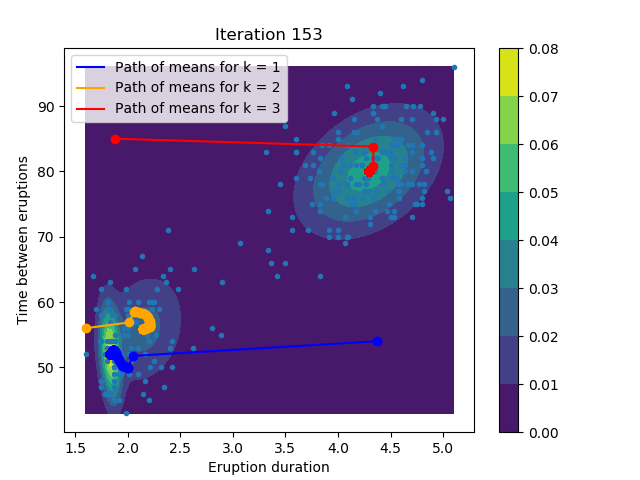
\includegraphics[width=\linewidth]{contourk3.png}\\
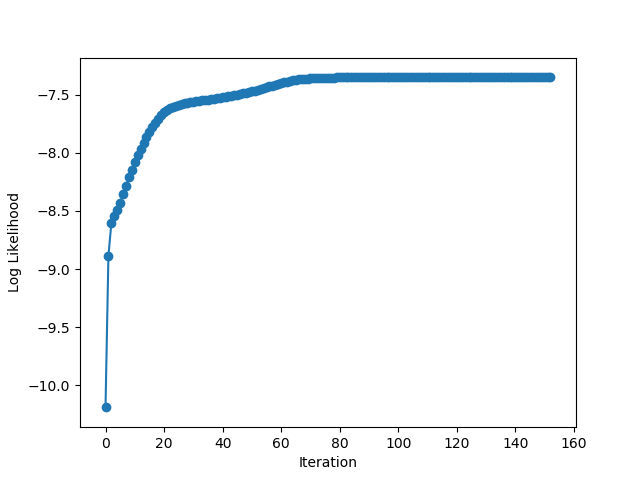
\includegraphics[width=0.75\linewidth]{log_likelihoodk3.png}
